\documentclass[12pt,letterpaper]{article}

% =====================
% Configuración general
% =====================
\usepackage[utf8]{inputenc}
\usepackage[T1]{fontenc}
\usepackage[spanish]{babel}
\usepackage{listings}
\usepackage{xcolor}
\usepackage{geometry}
\usepackage{setspace}
\usepackage{titlesec}
\usepackage{fancyhdr}
\usepackage{hyperref}
\usepackage{titlesec}
\usepackage{tabularx}
\usepackage{tocloft}
\usepackage{graphicx}
\usepackage{caption}
\usepackage{tocloft}
\usepackage{float}
\usepackage[backend=biber,style=apa,natbib=true]{biblatex}
% =====================
% --- Bloques de código ---
% =====================
% Definir colores para sintaxis Dart
\definecolor{keywordColor}{RGB}{0,0,180}   % azul para keywords
\definecolor{stringColor}{RGB}{163,21,21}  % rojo para strings
\definecolor{commentColor}{RGB}{0,128,0}   % verde para comentarios

% Configuración de listings para Dart
\lstdefinelanguage{Dart}{
  keywords={abstract, as, assert, async, await, break, case, catch, class, const,
            continue, covariant, default, defer, do, else, enum, export, extends,
            external, factory, false, final, finally, for, Function, get, if, implements,
            import, in, interface, is, late, library, mixin, new, null, on, operator,
            part, required, rethrow, return, set, show, static, super, switch, sync, 
            this, throw, true, try, typedef, var, void, while, with, yield},
  sensitive=true,
  comment=[l]{//},
  morecomment=[s]{/*}{*/},
  string=[b]",
}

\lstset{
  literate={á}{{\'a}}1
           {é}{{\'e}}1
           {í}{{\'i}}1
           {ó}{{\'o}}1
           {ú}{{\'u}}1
           {Á}{{\'A}}1
           {É}{{\'E}}1
           {Í}{{\'I}}1
           {Ó}{{\'O}}1
           {Ú}{{\'U}}1
           {ñ}{{\~n}}1
           {Ñ}{{\~N}}1
           {¡}{{!`}}1
           {¿}{{?`}}1,
  language=Dart,
  basicstyle=\ttfamily\fontsize{11}{13}\selectfont, % Consolas 11pt
  keywordstyle=\color{keywordColor}\bfseries,
  stringstyle=\color{stringColor},
  commentstyle=\color{commentColor}\itshape,
  showstringspaces=false,
  tabsize=4,
  breaklines=true,
  numbers=none,
  frame=single,
  rulecolor=\color{black},
  linewidth=\textwidth,
  framerule=0.1pt,
  xleftmargin=0pt,
  xrightmargin=0pt,
  captionpos=b
}

% Configuración de lstinline
\definecolor{inlinebg}{RGB}{240,240,240}       % gris claro
\definecolor{inlineborder}{RGB}{200,200,200}

\let\oldlstinline\lstinline
\renewcommand{\lstinline}[1]{%
  \colorbox{inlinebg!80!white}{%
    \setlength{\fboxsep}{1pt}%
    \textcolor{black}{\ttfamily\fontsize{11}{13}\selectfont #1}%
  }%
}

% =====================
% --- Bibliografía ---
% =====================
\addbibresource{ref.bib}  
\DeclareLanguageMapping{spanish}{spanish-apa}
\hypersetup{
    colorlinks=true,
    linkcolor=black,     % enlaces internos (capítulos, secciones) en negro
    citecolor=black,     % enlaces de citas en negro
    urlcolor=black       % enlaces de URLs en negro
}

% =====================
% --- Márgenes ---
% =====================
\geometry{
  top=2.54cm,
  bottom=2.54cm,
  left=3.17cm,
  right=3.17cm
}

% =====================
% --- Fuente Arial (Helvética) ---
% =====================
\usepackage{helvet}
\renewcommand{\familydefault}{\sfdefault}
\renewcommand\normalsize{\fontsize{11}{13}\selectfont}

% =====================
% --- Espaciado general ---
% =====================
\setstretch{1.5}
\setlength{\parindent}{0pt}
\setlength{\parskip}{16pt}

% =====================
% Encabezado y numeración
% =====================
\pagestyle{fancy}
\fancyhf{} % limpia encabezados/pies
\fancyhead[R]{\thepage} % número de página arriba a la derecha
\renewcommand{\headrulewidth}{0pt} % sin línea inferior

% =====================
% Colores institucionales
% =====================
\definecolor{azulOscuro}{RGB}{54,95,145}  % para Título1
\definecolor{azulClaro}{RGB}{79,129,189}  % para Título2
\definecolor{negro}{RGB}{0,0,0}

% =====================
% --- Formato de Figuras ---
% =====================
\captionsetup[figure]{
    labelfont={bf, color=azulClaro},
    textfont={color=azulClaro, small},
    justification=centering,
    labelsep=space
}

\graphicspath{{img/}}

% =====================
% Formato de Título1 (chapters) y Título2 (sections)
% =====================

% -- Título 1 --
\titleformat{\section}[hang]
  {\bfseries\color{azulOscuro}\fontsize{14}{16}\selectfont}
  {\thesection.}
  {1em}
  {}
\titlespacing*{\section}{0pt}{24pt}{{-16pt}}  % espaciado "antes" 24pt, "después" 12pt

% -- Título 2 --
\titleformat{\subsection}[hang]
  {\bfseries\color{azulClaro}\fontsize{12}{14}\selectfont}
  {\thesubsection.}
  {0.8em}
  {}
\titlespacing*{\subsection}{0pt}{10pt}{{-16pt}}  % espaciado "antes" 10pt, "después" 0pt

% =====================
% Índice de contenidos dinámico
% =====================
\setcounter{tocdepth}{2} % muestra capítulos y secciones en el índice
\hypersetup{
    colorlinks=true,
    linkcolor=negro,
    urlcolor=negro
}

% Hacer que las secciones tengan puntos hasta el número de página
\renewcommand{\cftsecleader}{\cftdotfill{\cftdotsep}}


% =====================
% Índice de figuras dinámico
% =====================
\renewcommand{\cftfigpresnum}{Ilustración\ }
\setlength{\cftfignumwidth}{3cm}
\renewcommand{\cftfigleader}{\cftdotfill{\cftdotsep}}

% =====================
% Documento
% =====================
\begin{document}
\renewcommand{\figurename}{Ilustración} 
{\textbf{\textcolor{azulOscuro}{INFORME LABORATORIO 2}}}

%===========================================================
%===========================================================
% --- Tabla de Datos ---
%===========================================================
%===========================================================

{\setlength{\parskip}{0pt}
\section{Datos Generales}
}

\begin{tabularx}{\textwidth}{|>{\raggedright\arraybackslash}X|>{\raggedright\arraybackslash}X|}
\hline
Título del Informe: & Creación y ejecución de un proyecto \\
\hline
Autor(a): & Carlos Hernández, Olivier Paspuel, Antonio Revilla, Frederick Tipán\\
\hline
Carrera: & Ingeniería en Software \\
\hline
Asignatura o Proyecto: & Aplicar Paradigma Atomic Desing y componentes UI \\
\hline
Tutor o Supervisor: & Mgtr. Doris Karina Chicaiza Angamarca\\
\hline
Institución: & Universidad de las Fuerzas Armadas ESPE – Matriz Sangolquí \\
\hline
Fecha de entrega: & 31 de octubre de 2025 \\
\hline
\end{tabularx}


%===========================================================
%===========================================================
% --- Introducción ---
%===========================================================
%===========================================================

\section{Introducción}

El siguiente informe presenta el desarrollo de 5 aplicaciones simples con validación básica, las cuales pueden ser ejecutadas mediante una pantalla de navegación principal. Por tal motivo, cada una de las aplicaciones hace uso de distintas pantallas, métodos de navegación y diferentes componentes visuales (widgets) para ejecutar su funcionalidad.

Para el desarrollo de cada uno de los ejercicios propuestos, se aplicó el patrón MVC. También se implementaron widgets reutilizables al basarse en Atomic Design, para lograr tener un diseño consistente por toda la aplicación. Adicionalmente, se agregó la librería de íconos “font awesome” para la implementación de elementos visuales variados en distintas pantallas. 

Los 5 ejercicios realizados, permitieron familiarizarse con distintas maneras de manejar la navegación entre vistas, así como el paso de argumentos entre componentes padre e hijo. También, el patrón MVC permitió mantener una base de código limpia y modular para reutilizar distintos componentes entre cada una de las aplicaciones.

\newpage

%===========================================================
%===========================================================
% --- índice de Contenidos y Figuras ---
%===========================================================
%===========================================================

\renewcommand{\contentsname}{Índice de Contenidos}
{\setlength{\parskip}{0pt}
\tableofcontents
}

\vspace{1.0cm}

\renewcommand{\listfigurename}{Índice de Ilustraciones}
{\setlength{\cftbeforefigskip}{2pt}
\listoffigures
}

\newpage

%===========================================================
%===========================================================
% --- Objetivos ---
%===========================================================
%===========================================================

\section{Objetivos}
\subsection{Objetivo General}
Elaborar un proyecto donde se puedan ejecutar 5 programas distintos en un entorno móvil con Flutter, las cuales implementen un mecanismo de navegación entre vistas.

\subsection{Objetivo Específicos}
- Mantener cosistencia entre las vistas mediante el uso widgets reutilizables con esquemas de color predefinidos.

- Hacer uso de estados para el manejo dinámico de la presentación de elementos visuales de la interfaz de usuario.

- Implementar navegabilidad entre distintas vistas de la aplicación mediante NavigationNamded con argumentos.

%===========================================================
%===========================================================
% --- Marco Teórico ---
%===========================================================
%===========================================================

\section{Marco Teórico}
\subsection{Paradigma Atomic Design}
MARCO TEORICO

%===========================================================
%===========================================================
% --- Desarollo ---
%===========================================================
%===========================================================

\section{Desarrollo}

El proyecto se encuentra cargado en el siguiente repositorio de GitHub: 

\href{https://github.com/vieerr/saint-roche-atomic-design}{\color{blue}\underline{https://github.com/vieerr/saint-roche-atomic-design}}

\subsection{Estrucutra de proyecto}

El archivo raiz del proyecto \lstinline{main.dart} se compone de las siguientes rutas con sus respectivas vistas:

\begin{center}
\begin{lstlisting}
routes: {
  '/': (context) => const Home(),
  '/bill': (context) => const BillScreen(),
  '/bill/result': (context) => const BillResultScreen(),
  '/products': (context) => ArticuloView(),
  '/teacher': (context) => TeacherView(),
  '/numbers': (context) => NumbersView(),
  '/hamburger': (context) => HamburgerScreen(),
  '/hamburger/result': (context) => HamburgerResult(),
},
\end{lstlisting}
\end{center}

\begin{figure}[H]
    \centering
    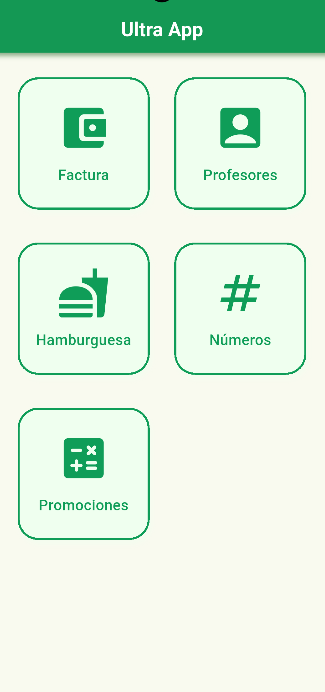
\includegraphics[width=0.7 \textwidth, height=9cm, keepaspectratio]{home_screen.png}
    \caption{Pantalla de inicio}
    \label{fig:home_screen}
\end{figure}

Para cada ejericio, se implementó el patrón MCV, por lo que se cuentan con las siguientes carpetas:

\begin{itemize}
    \item Controller
    \item Model
    \item View
    \item Widgets
\end{itemize}

El directorio de “widgets” es exclusivo para cada ejercicio, con componentes (widgets) específicos para implementar el ejercicio, aunque en algunos casos ciertos componentes se pueden compartir entre otros ejercicios.

Por ello, se cuenta con una carpeta general llamada \textbf{“commons”} en la que se colocan diversos componentes genéricos que pueden ser utilizados/compartidos por diferentes vistas.

\begin{figure}[H]
    \centering
    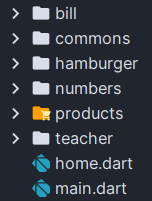
\includegraphics[width=0.4 \textwidth, height=6cm, keepaspectratio]{estructura_proyecto.png}
    \caption{Estructura general de proyecto}
    \label{fig:estructura_proyecto}
\end{figure}


\subsection{Problema 1}

\textit {“Desarrollo y explicación de problema 1 “Indicaciones al ejercicio en clase calcular el iva de 15\%, si las compras superan \textdollar2000 al cliente se agregar un descuento del 20\%, mostrar tanto el sueldo a ganar del vendedor y la factura de la venta de productos.”}

\textbf{Modelo}

Para desarrollar este ejercicio, se tienen 3 métodos en la clase del modelo.

\begin{center}
\begin{lstlisting}
  // Getter total ventas
  double get totalVentas => venta1 + venta2 + venta3;

  double calcularSueldo() {
    double sueldoBase = 36500;
    double comision = totalVentas * 0.12;
    return sueldoBase + comision;
  }

  double obtenerDescuento() {
    if(totalVentas >= 2000){
      return totalVentas * 0.20;
    }
    return 0;
  }
\end{lstlisting}
\end{center}

Las variables \lstinline{venta1}, \lstinline{venta2} y \lstinline{venta3} son atributos de la clase modal. Estas permiten obtener los valores del total de las ventas, un descuento si las ventas totales supera los \textdollar2000 y el sueldo del trabajador más su comisión del 12\% por cada venta.

\textbf{Controlador}

El controlador, toma este modelo y realiza las validaciones de texto correspondientes antes de ejecutar acciones sobre las variables numéricas de las ventas. En este método se retorna los valores respecto al total de las ventas, sueldo, descuento y el mensaje de error (en caso de haberlo).

\begin{center}
\begin{lstlisting}
  final billModel = BillModel(v1, v2, v3);
   final sueldo = billModel.calcularSueldo();
   final descuento = billModel.obtenerDescuento();

   return (billModel.totalVentas, sueldo, descuento, "");
\end{lstlisting}
\end{center}

\textbf{Vistas}

Dentro de la vista, una vez que se presiona el botón de calcular, se utiliza el controlador para mostrar obtener los resultados o los errores antes de realizar la acción. En caso de que todo fluya con normalidad, se pasan los datos a la ruta de resultados para mostrar los resultados en una nueva pantalla.

\begin{center}
\begin{lstlisting}
void _calcular() {
  final (totalVentas, sueldo, descuento, err) = mainctrl.calcularDatos(
      venta1ctrl.text,
      venta2ctrl.text,
      venta3ctrl.text,
  );

  // actualizar mensaje de error
  setState(() {
    msgErr = err;
  });

  // no mostrar pasar a la siguiente pantalla si hubo un error
  if(err != "") {
    return;
  }

  Navigator.pushNamed(
      context, "/bill/result",
      arguments: {
        'totalVentas': totalVentas,
        'sueldo': sueldo,
        'descuento': descuento,
      }
  );
}
\end{lstlisting}
\end{center}

Puesto que se mandaron argumentos en forma de clave valor, se realizaron colocaron los siguientes comandos para obtener cada uno de los argumentos en la vista de resutlados.

\begin{center}
\begin{lstlisting}
  @override
  Widget build(BuildContext context) {
    final args = ModalRoute.of(context)!.settings.arguments as Map<String, double>;

    final double totalVentas = args['totalVentas']!;
    final double sueldo = args['sueldo']!;
    final double descuento = args['descuento']!;
  }
\end{lstlisting}
\end{center}

\textbf{Ejecución}

De esta manera se pudo cumplir con el ejercicio propuesto, donde se toman 3 valores y con ellos se realizan varios cálculos mostrados en la siguiente pantalla:

\begin{figure}[H]
    \centering
    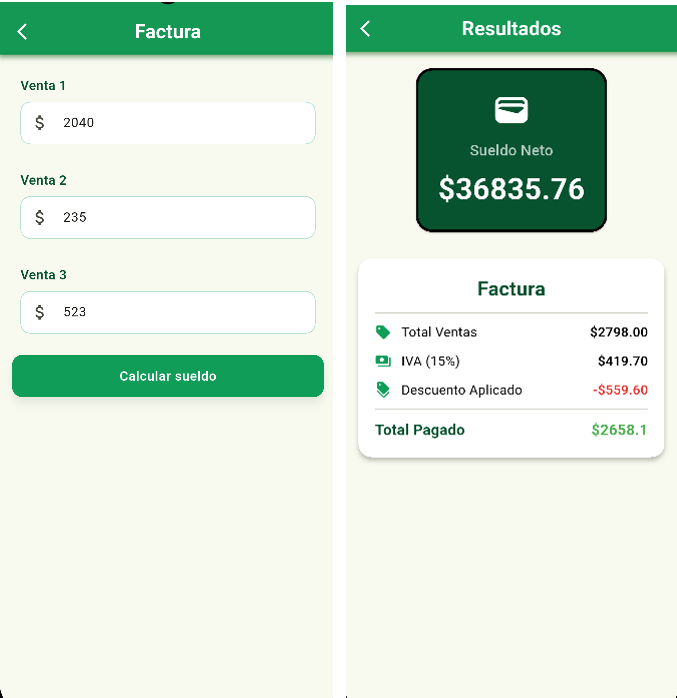
\includegraphics[width=0.8 \textwidth, height=10cm, keepaspectratio]{ejecucion_ej1.png}
    \caption{Ejecucción ejercicio 1}
    \label{fig:ej1_ejecuccion}
\end{figure}
\subsection{Problema 2}

\textit {“Un profesor tiene un salario inicial de \$1500, y percibe un incremento de 10\% anual durante 6 años. ¿Cuál es su salario al cabo de 6 años? ¿Qué salario ha recibido en cada uno de los 6 años?”}

\textbf{Modelo}

En el modelo se especifican 3 atributos para realizar los cálculos. Siendo estos:

\begin{center}
\begin{lstlisting}
final double salarioInicial;
final double incremento;
final int anios;
\end{lstlisting}
\end{center}

Así, se las incorporarían dentro de un método para calcular los salarios del profesor a través de 5 años (ya que el primer año es el salario inicial). Para ello se va armando una lista donde se multiplica por 0.10 el salario actual de la persona.

\begin{center}
\begin{lstlisting}
List<double> calcularSalarios() {
  List<double> salarios = [salarioInicial];
  double actual = salarioInicial;

  for (int i = 1; i <= anios; i++) {
    actual += actual * incremento;
    salarios.add(double.parse(actual.toStringAsFixed(2)));
  }

  return salarios;
}
\end{lstlisting}
\end{center}

Finalmente, se obtiene el salario final de la persona, al tomar el último elemento de la lista.

\begin{center}
\begin{lstlisting}
double obtenerSalarioFinal() {
  return calcularSalarios().last;
}
\end{lstlisting}
\end{center}

\textbf{Controlador}

El controlador hace uso del modelo anterior. En este caso, la función devuelve un \lstinline{Map$<>$} que tiene dos argumentos: la lista de salarios y el salario final.

\begin{center}
\begin{lstlisting}
Map<String, dynamic> calcularSalarios(String salarioStr){ ... }
\end{lstlisting}
\end{center}

Para ello, primero se trata de verificar que el valor \lstinline{String} suministrado pueda ser convertido a un número decimal, de no ser el caso se retorna un mensaje de error.

\begin{center}
\begin{lstlisting}
try {
  double salario = double.parse(salarioStr);
  ...
} catch (e) {
  return {
  'error': "Ingresa un número válido para el salario inicial."
  };
}
\end{lstlisting}
\end{center}

Luego se utiliza el modelo, definiendo el salario inicial y calculando los salarios, por lo que al final se retorna tanto la lista de salarios como el salario final.

\begin{center}
\begin{lstlisting}
  final modelo = SalarioModel(salarioInicial: salario);
  final lista = modelo.calcularSalarios();

  return {
    'salarios': lista,
    'salarioFinal': modelo.obtenerSalarioFinal(),
  };
\end{lstlisting}
\end{center}

\textbf{Vistas}

En la vista principal, se hace uso de 3 variables para manejar el estado: el controlador, un mensaje de eror y el campo de texto del input. Con estas 3 variables, se las usa en la función \lstinline{calcular()}. En donde se realizan validaciones previas antes de utilizal el método del controlador y pasar a la siguiente pantalla de resutlados, donde se le pasa el \lstinline{Map} como argumento.

\begin{center}
\begin{lstlisting}
void calcular() {
    setState(() {
      errorMessage = null;
    });

    final input = salarioCtrl.text.trim();

    if (input.isEmpty) {
      setState(() {
        errorMessage = "Por favor, ingresa un salario inicial.";
      });
      return;
    }

    final salario = double.tryParse(input);

    if (salario == null) {
      setState(() {
        errorMessage = "El salario debe ser un número válido (sin letras ni símbolos).";
      });
      return;
    }

    if (salario <= 0) {
      setState(() {
        errorMessage = "El salario debe ser mayor que cero.";
      });
      return;
    }

    final resultado = controller.calcularSalarios(salarioCtrl.text);
    Navigator.pushNamed(context, 'teacher/result', arguments: resultado);
  }
\end{lstlisting}
\end{center}

Luego, en la vista de resultados, se recuperan los argumentos de la siguiente manera:

\begin{center}
\begin{lstlisting}
final resultado = ModalRoute.of(context)!.settings.arguments as Map<String, dynamic>;

final List<double>? salarios = resultado['salarios'] as List<double>?;
final double? salarioFinal = resultado['salarioFinal'] as double?;
\end{lstlisting}
\end{center}

\textbf{Ejecución}

De esta manera se pudo cumplir con el ejercicio propuesto, donde se dan a los 6 años de salario del profesor con un incremento del 10\% anual mediante las siguientes pantallas:

\begin{figure}[H]
    \centering
    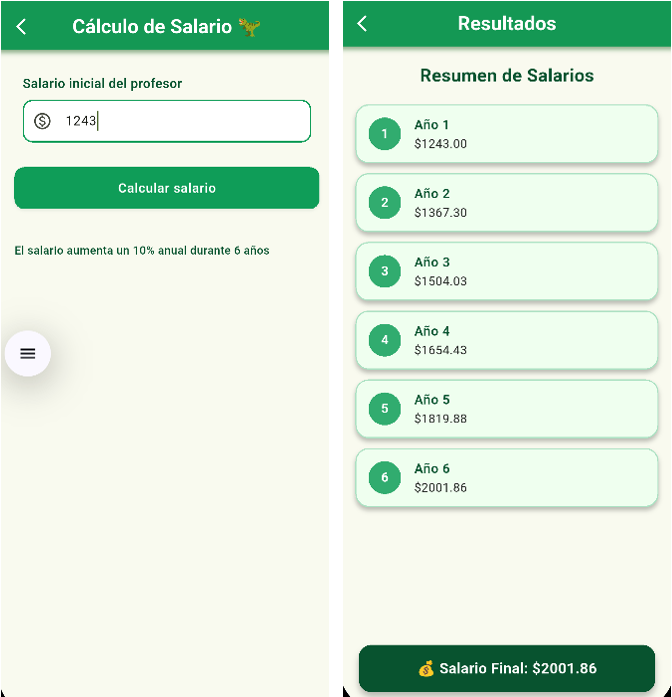
\includegraphics[width=0.8 \textwidth, height=8cm, keepaspectratio]{ejecucion_ej2.png}
    \caption{Ejecucción ejercicio 2}
    \label{fig:ej2_ejecucion}
\end{figure}
\subsection{Problema 3}

\textit {“El náufrago satisfecho ofrece hamburguesas sencillas (S), dobles (D) y triples (T), las cuales tienen un costo de \$20, \$25 y \$28 respectivamente. La empresa acepta tarjetas de crédito con un cargo de 5\% sobre la compra. Suponiendo que los clientes adquieren N hamburguesas, las cuales pueden ser de diferente tipo, realice un algoritmo para determinar cuánto deben pagar.”}

\textbf{Modelo}

Puesto que se tienen 3 opciones predefinidas, se optó por realizar un \lstinline{enum} con las 3 opciones especificadas.

\begin{center}
\begin{lstlisting}
enum HamType {
  sencilla('Sencilla', 20),
  doble('Doble', 25),
  triple('Triple', 28);

  final String name;
  final double price;
  const HamType(this.name, this.price);
}
\end{lstlisting}
\end{center}

Con este enum, se lo utilizó dentro del modelo, donde se especifica una cantidad para cada tipo de hamburguesa. Adicionalmente se tienen los métodos para calular el total tomando en cuenta el precio base y la cantidad correspondiente.

\begin{center}
\begin{lstlisting}
class HamburgerModel {
  final HamType hamburger;
  int quantity;

  HamburgerModel({required this.hamburger, this.quantity = 0});

  double get total => hamburger.price * quantity;
}
\end{lstlisting}
\end{center}

\textbf{Controlador}

Primero se tiene una lista con el modelo, por lo que se lo transforma mediante:

\begin{center}
\begin{lstlisting}
final List<HamburgerModel> hamburgers = [
  for(var ham in HamType.values)
    HamburgerModel(hamburger: ham)
];
\end{lstlisting}
\end{center}

Luego se definieron métodos para aumentar y disminuir la cantidad de un determinado tipo de hamburguesa. Estos métodos serán utilizados por los widgets \lstinline{Counter} para mostrar en pantalla la cantidad actual de cada hamburguesa.

\begin{center}
\begin{lstlisting}
  void increaseQty(HamburgerModel ham) {
    ham.quantity++;
  }

  void decreaseQty(HamburgerModel ham) {
    if (ham.quantity > 0) {
      ham.quantity--;
    }
  }
\end{lstlisting}
\end{center}

Luego se tienen los métodos para calcular el total a pagar, esto se lo hace recorriendo la lista principal y llamando al método \lstinline{total} para sumar acumulativamente los valores.

\begin{center}
\begin{lstlisting}
double get total {
  double hamTotal = 0;
  for(int i=0; i<hamburgers.length; i++) {
    hamTotal += hamburgers[i].total;
  }
  return hamTotal;
}
\end{lstlisting}
\end{center}

Luego, en caso de que se tenga recargo por la tarjeta de crédito, se obtiene el valor del recargo en base al total de toda la venta. Adicionalmente se tiene con un método que verifica si no se ha seleccionada ninguna hamburguesa, si este es el caso, se devolverá un mensaje de error.

\begin{center}
\begin{lstlisting}
double get charge {
    return total * RECARGO;
  }

String allHamburgersZero() {
  for(int i=0; i<hamburgers.length; i++){
    if(hamburgers[i].quantity != 0) {
      return "";
    }
  }
  return "Agregue por lo menos una hamburguesa";
}
\end{lstlisting}
\end{center}

\textbf{Vistas}

Dentro de la vista, se utiliza el controlador, junto con variables para el manejo del mensaje de error y si se ha aplicado el método de pago por tarjeta de crédito.

\begin{center}
\begin{lstlisting}
final hamCtrl = HamburgerController();
bool _isCreditCardPayment = false;
String _errMsg = "";
\end{lstlisting}
\end{center}

Cuando el usuario presiona el botón para calcular el pago se utiliza el controlador, luego se verifica si se ha seleccionado al menos una hamburguesa, luego se comprueba si hay un recargo si se pagó con tarjeta de crédito, para finalmente pasar a la pantalla de resutlados con los argumentos correspondientes.

\begin{center}
\begin{lstlisting}
void _computeAllHamburgers() {
 setState(() {
   _errMsg = hamCtrl.allHamburgersZero();
 });

  if(_errMsg != "") {
    return;
  }

  double charge = 0;
  if(_isCreditCardPayment){
    charge = hamCtrl.charge;
  }

  Navigator.pushNamed(
    context, "/hamburger/result",
    arguments: {
      'total': hamCtrl.total,
      'recargo': charge,
      'hamburgesas': hamCtrl.hamburgers,
    }
  );
}
\end{lstlisting}
\end{center}

Luego, en la pantalla de resultados, se recuperaron los argumentos mediante:

\begin{center}
\begin{lstlisting}
final args = ModalRoute.of(context)!.settings.arguments as Map<String, dynamic>;

final double total = args['total']!;
final double recargo = args['recargo']!;
final List<HamburgerModel> hamburguesas = args['hamburgesas']!;
\end{lstlisting}
\end{center}

\textbf{Ejecución}

De esta manera se pudo cumplir con el ejercicio propuesto, donde se dan a mostrar 3 opciones de hamburguesa con la posibilidad de poder realizar el pago con tarjeta con una comisión adicional mediante las siguientes pantallas:

\begin{figure}[H]
    \centering
    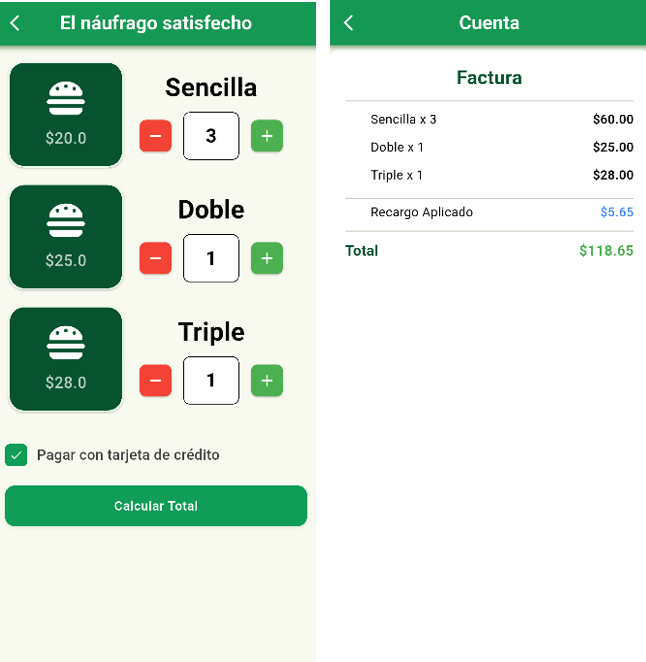
\includegraphics[width=0.8 \textwidth, height=10cm, keepaspectratio]{ejecucion_ej3.png}
    \caption{Ejecucción ejercicio 3}
    \label{fig:ej3_ejecuccion}
\end{figure}
\subsection{Problema 4}

\textit {"Se requiere un algoritmo para determinar, de N cantidades, cuántas son de cero, cuántas son menores a cero, y cuántas son mayores a cero."}

\textbf{Modelo}

El modelo recibe una lista de números y cuenta cuántos son ceros, negativos y positivos. Para ello se definen tres getters que recorren la lista.

\begin{center}
\begin{lstlisting}
int get zeros {
  int count = 0;
  for (int i = 0; i < numbers.length; i++) {
    if (numbers[i] == 0) {
      count++;
    }
  }
  return count;
}

int get negatives {
  int count = 0;
  for (int i = 0; i < numbers.length; i++) {
    if (numbers[i] < 0) {
      count++;
    }
  }
  return count;
}

int get positives {
  int count = 0;
  for (int i = 0; i < numbers.length; i++) {
    if (numbers[i] > 0) {
      count++;
    }
  }
  return count;
}
\end{lstlisting}
\end{center}

Cada getter itera sobre la lista de números y verifica la condición correspondiente, incrementando un contador cuando se cumple.

\textbf{Controlador}

El controlador valida los datos ingresados antes de procesarlos. Primero verifica que se haya ingresado la cantidad de números a procesar.

\begin{center}
\begin{lstlisting}
if (cantidad.isEmpty) {
  String err = "Ingrese la cantidad de números";
  return (0, 0, 0, err);
}

final n = int.tryParse(cantidad);

if (n == null) {
  String err = "Ingrese un valor numérico válido";
  return (0, 0, 0, err);
}

if (n <= 0) {
  String err = "La cantidad debe ser mayor a cero";
  return (0, 0, 0, err);
}
\end{lstlisting}
\end{center}

Luego valida que se hayan ingresado exactamente la cantidad de valores indicada y que todos sean numéricos.

\begin{center}
\begin{lstlisting}
if (valores.length != n) {
  String err = "Debe ingresar exactamente $n números";
  return (0, 0, 0, err);
}

List<double> numeros = [];
for (int i = 0; i < valores.length; i++) {
  if (valores[i].isEmpty) {
    String err = "Complete todos los campos";
    return (0, 0, 0, err);
  }

  final valor = double.tryParse(valores[i]);
  if (valor == null) {
    String err = "Ingrese valores numéricos válidos";
    return (0, 0, 0, err);
  }

  numeros.add(valor);
}
\end{lstlisting}
\end{center}

Finalmente, crea una instancia del modelo y retorna los resultados.

\begin{center}
\begin{lstlisting}
final model = NumbersModel(numeros);
return (model.zeros, model.negatives, model.positives, "");
\end{lstlisting}
\end{center}

\textbf{Vistas}

La vista principal permite ingresar la cantidad de números a procesar. Al presionar el botón de generar campos, se crean dinámicamente los inputs necesarios.

\begin{center}
\begin{lstlisting}
void _actualizarCantidad() {
  final n = int.tryParse(cantidadCtrl.text);
  if (n != null && n > 0 && n <= 20) {
    setState(() {
      cantidad = n;
      valoresCtrl = List.generate(n, (index) => TextEditingController());
      msgErr = "";
    });
  } else if (n != null && n > 20) {
    setState(() {
      msgErr = "La cantidad no puede ser mayor a 20";
      cantidad = 0;
      valoresCtrl = [];
    });
  }
}
\end{lstlisting}
\end{center}

Una vez ingresados todos los valores, se procesan mediante el controlador.

\begin{center}
\begin{lstlisting}
void _calcular() {
  List<String> valores = valoresCtrl.map((c) => c.text).toList();
  final (zeros, negatives, positives, err) = ctrl.procesarNumeros(
    cantidadCtrl.text,
    valores,
  );

  setState(() {
    msgErr = err;
  });

  if (err != "") {
    return;
  }

  Navigator.pushNamed(
    context,
    "/numbers/result",
    arguments: {
      'zeros': zeros,
      'negatives': negatives,
      'positives': positives,
    },
  );
}
\end{lstlisting}
\end{center}

En la pantalla de resultados, se obtienen los argumentos pasados y se muestran en una tarjeta con el conteo de cada categoría.

\begin{center}
\begin{lstlisting}
@override
Widget build(BuildContext context) {
  final args = ModalRoute.of(context)!.settings.arguments as Map<String, int>;

  final int zeros = args['zeros']!;
  final int negatives = args['negatives']!;
  final int positives = args['positives']!;
  final int total = zeros + negatives + positives;
}
\end{lstlisting}
\end{center}

\textbf{Ejecución}

El ejercicio permite ingresar N cantidades y clasifica cada una según su valor. Los resultados muestran cuántos números son cero, menores a cero y mayores a cero.


\subsection{Problema 5}

\textit {“Realice un algoritmo para determinar cuánto pagará una persona que adquiere N artículos, los cuales están de promoción. Considere que si su precio es mayor o igual a \$200 se le aplica un descuento de 15\%, y si su precio es mayor a \$100 pero menor a \$200, el descuento es de 12\%; de lo contrario, sólo se le aplica 10\%. Se debe saber cuál es el costo y el descuento que tendrá cada uno de los artículos y finalmente cuánto se pagará por todos los artículos obtenidos.”}




%===========================================================
%===========================================================
% --- Conclusiones y Recomendaciones ---
%===========================================================
%===========================================================

\section{Conclusiones y Recomendaciones}
\subsection{Conclusiones}
\begin{itemize}
    \item La realización del laboratorio permitió aplicar el patrón de diseño MVC, y también la metodología Atomic Design, lo cual permitió tener un proyecto con una estructura organizada, clara y adaptable para las distintas soluciones que se proponen para los problemas del laboratorio.
    
    \item El desarrollo del proyecto utilizando widgets reutilizables y esquemas de color uniformes permitió desarrollar un proyecto con coherencia visual en todas las soluciones que se plantean; esto facilitó la creación de las plantillas consistentes y mejoró la experiencia de usuario.

    \item El uso de la navegación entre vistas para poder visitar las diferentes soluciones planteadas con el uso de widgets reutilizables demostró mayor flexibilidad para el desarrollo de este proyecto; además, se logró mantener una comunicación entre los diferentes componentes y el flujo lógico dentro de la app desarrollada.
\end{itemize}

\subsection{Recomendaciones}
\begin{itemize}
    \item Se recomienda aplicar patrones de diseño y metodologías como MVC y Atomic Design en otros proyectos para poder tener un desarrollo limpio, modular y fácilmente escalable, lo que permite ofrecer un producto de mayor calidad.

    \item Se recomienda hacer uso de widgets que puedan ser más personalizados y temáticos, ya que estos permiten generar componentes que son más reutilizables, además de que fortalecen la identidad visual y reducen la redundancia de código para tener un código más limpio y de mejor calidad.
    
    \item Se recomienda profundizar en las diferentes opciones de navegación que Flutter ofrece, además de las diferentes opciones de manejo de estados, para poder optimizar el rendimiento y mejorar la interacción entre las diferentes pantallas del proyecto.
\end{itemize}

%===========================================================
%===========================================================
% --- Referencias Bibliográficas ---
%===========================================================
%===========================================================

\section{Referencias Bibliográficas}
\printbibliography[heading=none]

%===========================================================
%===========================================================
% --- Anexos ---
%===========================================================
%===========================================================

\section{Anexos}

\textbf{Manejo de errores}

\begin{figure}[H]
    \centering
    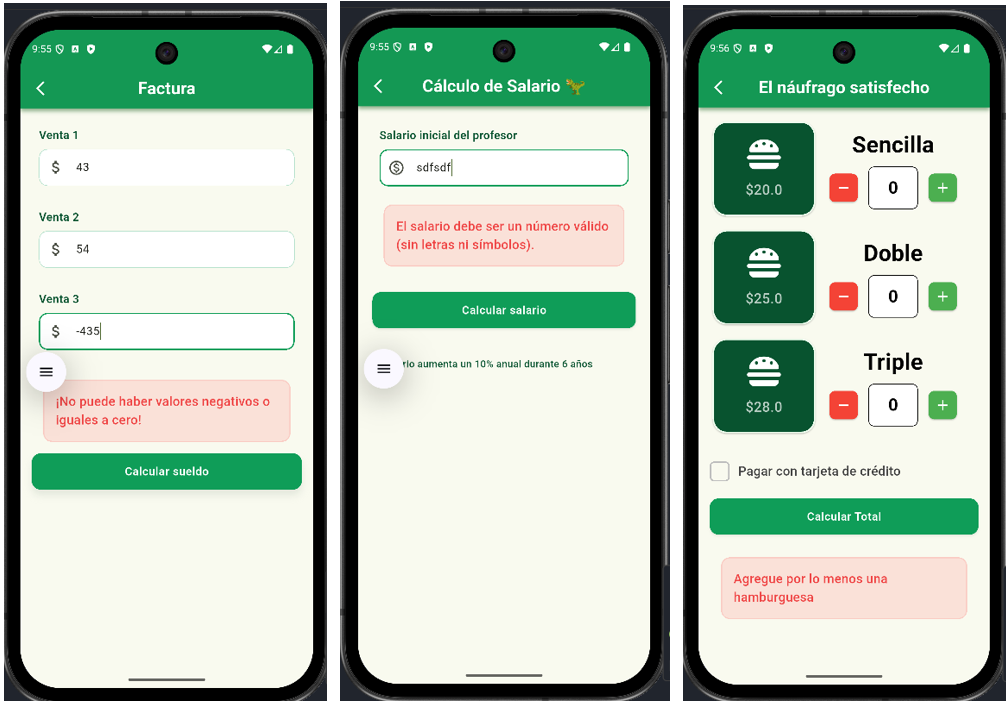
\includegraphics[width=0.8 \textwidth, height=10cm, keepaspectratio]{anexos/err_ejecucion.png}
\end{figure}

\end{document}
